\documentclass[a4paper,german,12pt,smallheadings]{scrartcl}
\usepackage[T1]{fontenc}
\usepackage[utf8]{inputenc}
\usepackage{babel}
\usepackage{geometry}
\usepackage{tikz}
\usepackage{wrapfig}
\usepackage[fleqn]{amsmath}
\usepackage{amssymb}
\usepackage{float}
\usepackage{enumerate}
\usepackage{listings} % Source code
\usepackage{lscape} % landscape
\usepackage{commath} % http://tex.stackexchange.com/questions/14821/whats-the-proper-way-to-typeset-a-differential-operator
\usepackage{cancel}
\usepackage[fleqn]{mathtools}
% Number only referenced equations
%\mathtoolsset{showonlyrefs}

%\usepackage{wrapfig}
\usepackage{siunitx}
\sisetup{separate-uncertainty=true,locale=DE}

% New command for color underlining
\usepackage{xcolor}
\newcommand\invisiblesection[1]{%
    \refstepcounter{section}%
      \addcontentsline{toc}{section}{\protect\numberline{\thesection}#1}%
        \sectionmark{#1}}
\newsavebox\MBox
\newcommand\colul[2][red]{{\sbox\MBox{$#2$}%
  \rlap{\usebox\MBox}\color{#1}\rule[-1.2\dp\MBox]{\wd\MBox}{0.5pt}}}

\restylefloat{table}
\geometry{a4paper, top=15mm, left=20mm, right=10mm, bottom=20mm, headsep=10mm, footskip=12mm}
\linespread{1.5}
\setlength\parindent{0pt}
\DeclareMathOperator{\Tr}{Tr}
\DeclareMathOperator{\Var}{Var}
\begin{document}

\begin{titlepage}
\newcommand{\HRule}{\rule{\linewidth}{0.5mm}}

\begin{center}
  \textsc{\Large Physikalisches Grundpraktkum 1}
  \HRule\\[0.4 cm]
  {\huge \bfseries Gleichmäßig beschleunigte Drehbewegungen}
  \HRule\\[0.4 cm]

  \begin{minipage}{0.65\textwidth}
  \begin{flushleft}
    Markus Fenske \texttt{<iblue@zedat.fu-berlin.de>} \\
    Paul Rahmann \texttt{<paulrahmann@zedat.fu-berlin.de>}
  \end{flushleft}
  \end{minipage}
  \hfill
  \begin{minipage}{0.30\textwidth}
  \begin{flushright}
    Tutor: Christian Hindermann \\
    Versuchstag: 6. Juni 2014
  \end{flushright}
  \end{minipage}

  \vspace{1cm}

  \tableofcontents


  %{\large \today}
  \vfill
\end{center}
\newpage

\end{titlepage}

\allowdisplaybreaks % Seitenumbrüche in Formeln erlauben
\begin{center}
\bfseries % Fettdruck einschalten
\sffamily % Serifenlose Schrift
\vspace{-40pt}
Physikalisches Grundpraktikum 1, Sommersemester 2014

Markus Fenske \texttt{<iblue@zedat.fu-berlin.de>}

Paul Rahmann \texttt{<paulrahmann@zedat.fu-berlin.de>}

Drehbewegungen, Tutor: Christian Hindermann
\vspace{-10pt}
\end{center}

\section{Physikalische Grundlagen}
Das Trägheitsmoment wird durch $F = \dot{p} = m \dot{v}$ motiviert. Wenn auf eine Masse $m$
im Abstand $r$ von der Drehachse eine Kraft wirkt, folgt

\begin{equation}
  \vec{r} \times \vec{F}
  = \vec{r} \times m \dot{\vec{v}}
\end{equation}

mit $v = r \omega$ und $r$ konstant und weil die Drehachse senkrecht auf Kraft
und Ortsvektor steht

\begin{equation}
  = \dot{\vec{\omega}} r^2 m
\end{equation}

Durch Überführung von $m$ in ein Massenelement $\dif m$ folgt

\begin{equation}
  \underbrace{\vec{r} \times \vec{F}}_{=: \vec{M}} = \dot{\vec{\omega}} \underbrace{\int \dif m \; r^2}_{=: I}
\end{equation}

Wir verwenden ab hier nur die Beträge, da alle Vektoren jeweils senkrecht
aufeinander stehen. Die Richtungen können dann aus der Rechte-Hand-Regel
ermittelt werden.

Die Bewegungsgleichung für die Drehbewegung eines starren Körpers lautet also gemäß der Herleitung
\begin{equation}
  M = I \dot{\omega} = I \ddot{\phi}
\end{equation}

Analog zur Newtonschen Bewegungsgleichung für lineare Bewegungen unter Einfluss
einer konstanten Kraft ist die Lösung dieser Differentialgleichung unter
Annahme eines konstanten Drehmoments $M$
\begin{equation}
  \phi(t) = \frac{M}{2I}t^2 + \omega_0 t + \phi_0
  \label{eq_of_motion}
\end{equation}

Dabei ist $M$ das konstante Drehmoment, $I$ das Trägheitsmoment, $\omega_0$ die
Anfangswinkelgeschwindigkeit und $\phi_0$ der Anfangswinkel. Als Konsequenz
ergibt sich unter Einfluss einer konstanten Kraft also eine lineare Zunahme der
Winkelgeschwindigkeit
\begin{equation}
  \omega(t) = \frac{M}{I} t + \omega_0
\end{equation}

Das Drehmoment im Schwerpunktkoordinatensystem ist

\begin{equation}
  I = \int \dif m \; r^2
  \label{speed}
\end{equation}

Sei die Drehachse oBdA $\omega \hat{z}$. Verschieben wir die Drehachse um
$(a_x, a_y)$ erhalten wir

\begin{align*}
  I_a &= \int \dif m \; \del{(x - a_x)^2 + (y - a_y)^2} \\
      &= \int \dif m \; \del{x^2 - 2xa_x + a_x^2 + y^2 - 2ya_y + a_y^2} \\
      &= \int \dif m \; \del{x^2 + y^2}
       + 2 a_x \int \dif m \; x
       + 2 a_y \int \dif m \; y
       + \del{a_x^2 + a_y^2} \int \dif m
\end{align*}

Der erste Term ist das Drehmoment um den Schwerpunkt, die nächsten beiden
Integrale sind die $x$- und die $y$-Koordinate des Schwerpunktes im
Schwerpunktsystem. Da in diesem der Schwerpunkt im Ursprung liegt, verschwinden
sie. Das nächste Integral ist einfach die Gesamtmasse. Somit

\begin{equation}
  I_a = I + ma^2
\end{equation}

Dies ist der Steinersche Satz.

Für die Aufgabenstellung ist außerdem die Berechnung des Trägheitsmoments eines
starren Zylinders gefordert. Ein Vollzylinder wird dem experimentellen Aufbau
nicht gerecht, denn die Masse konzentriert sie unseren Erachtens nach auf den
Reifen, nicht auf die Speichen. Gehen wir also von einer Massenverteilung $\rho
= \frac{m}{2 \pi R} \delta(r-R)\delta(z)$ aus, erhalten wir

\begin{equation}
  I = \int \dif V \; r^2 \rho = m R^2
\end{equation}

\section{Aufgaben}
%Untersuchung gleichmäßig beschleunigter Drehbewegungen
%\begin{itemize}
%  \item Messung von Weg-Zeit-Abhängigkeiten
%  \item Messung von Drehmoment-Zeit-Abhängigkeiten
%  \item Messung der Reibungsverluste
%\end{itemize}
%für unterschiedliche Trägheitsmomente (mit und ohne Zusatzmassen).
\begin{enumerate}[1.]
  \item Qualitative und quantitative Überprüfung des Bewegungsgesetzes. Messung
    der Zeit in Abhängigkeit des Drehwinkels (bei festem Drehmoment) und in
    Abhängigkeit des Drehmoments (bei festem Drehwinkel). Bestimmung der
    Trägheitsmomente (mit und ohne Zusatzmassen) des Rades aus den Messungen
    und Vergleich mit dem berechneten Wert aus dem \textit{Steinerschen Satz}.
  \item
    Diskussion von Reibungseinflüssen und Reibungsmodellen (Abhängigkeit von
    Reibungskräften bzw. Reibungsmomenten von den verschiedenen
    Bewegungsparametern) aus den Ergebnissen der Messungen.
\end{enumerate}

\newpage
\invisiblesection{Durchführung und Auswertung}
\subsection{Versuchsaufbau}
\begin{wrapfigure}{R}{10.1 cm}
  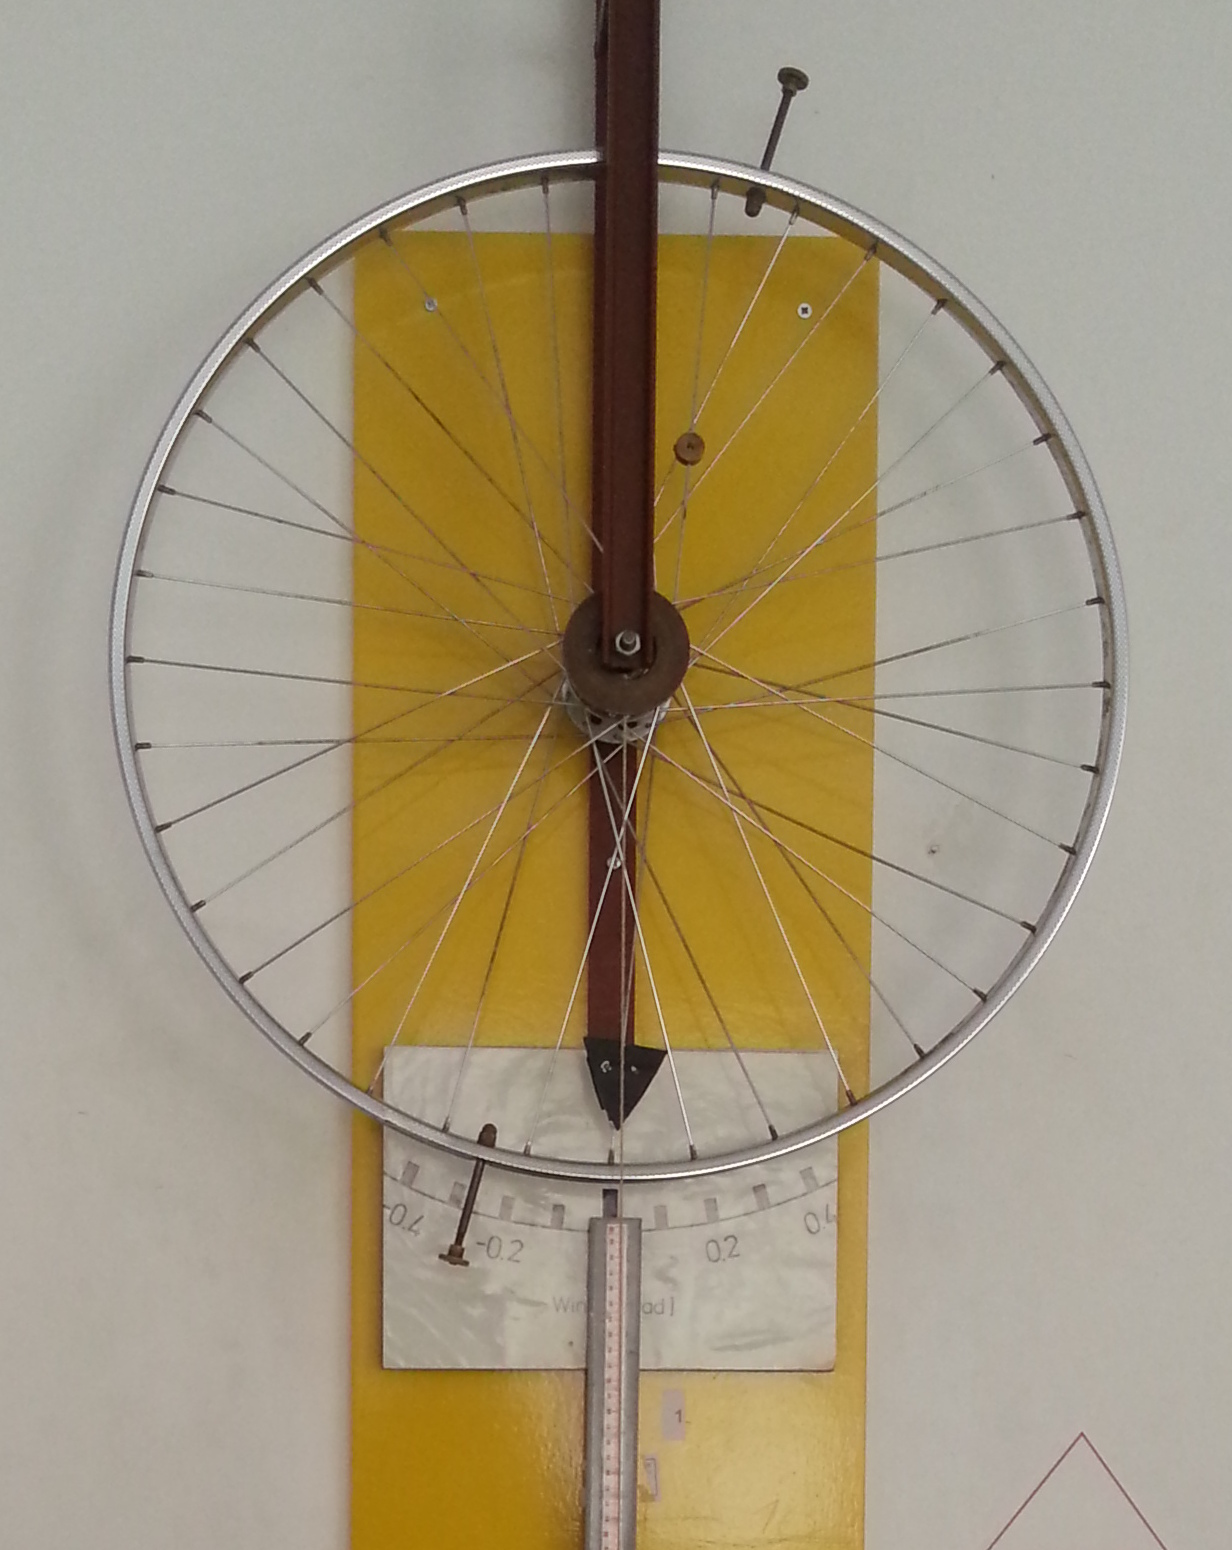
\includegraphics[width=10cm]{fig1.jpg}
  \caption{Versuchsaufbau}
\end{wrapfigure}
Das Rad eines Fahrrads ist drehbar an der Wand montiert. Auf seiner Achse
befindet sich eine Rolle, auf der eine Schnur aufgewickelt wird. Am Ende
der Schnur hängt eine Feder, an die verschiedene Gewichte angehängt werden
können. Wird das Rad losgelassen folgt das Gewicht der Schwerkraft und dreht
dadurch das Rad.

Das Rad verfügt über einen radialen Zeiger, der den Drehwinkel des Rades auf
einer Skala anzeigt. Die Skala geht nur von von ca. $-0{,}4$ rad bis $0{,}4$
rad, umfasst also nur einen kleinen Winkel von etwa $50\,^\circ$.  Im
restlichen Bereich kann der Winkel nur grob geschätzt werden.

Es gibt außerdem eine Skala zum Ablesen der Höhe des Gewichts, wir wir jedoch
aus nicht verwendet haben. Stattdessen haben wir die Höhe aus der
Zeigerposition geschätzt.

Am Rad befinden sich außerdem zwei Gewindestangen auf gegenüberliegenden
Seiten. An ihnen können mit Rändelmuttern zwei zusätzliche Gewichte befestigt
werden, um das Trägheitsmoment des Rades zu erhöhen.

\subsection{Versuchsdurchführung}

Wir haben ein Gewicht angehängt, eine bestimmte Anzahl Umdrehungen aufgewickelt
und dann das Rad losgelassen. Das Gewicht wird von der Schwerkraft nach unten
gezogen und bringt dadurch das Rad in eine Drehbewegung. Sobald die Schnur
komplett abgewickelt ist (Umkehrpunkt), zieht das Rad das Gewicht wieder nach
oben, bis es an einem zweiten Hochpunkt wieder zum Stillstand kommt.

Mit einer Stoppuhr haben wir parallel zwei Zeiten gemessen. Der erste Messwert
ist die Zeit, die vom Hoch- zum Umkehrpunkt verstreicht. Der zweite Messwert ist
die Zeit vom Hoch- zum nächsten Hochpunkt.

Die Höhe des zweiten Hochpunkts des Gewichtes haben wir abgeschätzt, indem wir
die noch aufgewickelten Umdrehungen und die ungefähre Position des Zeigers
(Angaben von 0 bis 12 Uhr) abgeschätzt haben.

Mit den 5 verschiedenen Anhängemassen, den zwei verschiedenen Drehrichtungen
(im und gegen den Uhrzeigersinn) und in der Konfiguration mit und ohne
Zusatzmassen haben wir Messreihen für 1, 2 und 5 Umdrehungen aufgenommen. So
haben wir 60 Messwertreihen mit jeweils 2 Zeiten erhalten.

Außerdem haben wir jede Messung mit der Handykamera (Samsung Galaxy S3,
mp4-Format, variable Framerate) aufgenommen um die abgeschätzten Positionen und
evtl. Zeiten zu verfeinern oder vielleicht weitere Daten extrahieren zu können.

\subsection{Datenanalyse}
Da es uns wenig herausfordernd und monoton erschien, die aufgenommenen Videos
manuell zu analysieren, haben wir zu diesem Zweck eine Software entwickelt,
deren Funktionsweise in Kapitel~\ref{chap:software} ab
Seite~\pageref{chap:software} genauer erklärt ist.

Die Software extrahiert automatisch aus den Videos die jeweilige Position des
Zeigers (Winkel) in Abhängigkeit von der Zeit.

Wir konnten damit für 33 der 60 Messungen eine sehr genaue Ort-Zeit-Kurve
erstellt. Insgesamt haben wir über 38.000 Messpunkte extrahiert.

\subsection{Aufgabe 2}
Da man anhand der Messwerte sofort sehen kann (siehe Plot 1 auf
Seite~\pageref{plot:57-lin}), dass die ursprünglich hergeleitete
Bewegungsgleichung (überhaupt nicht zutrifft, bearbeiten wir zuerst Aufgabe 2.

Aus der Bewegungsgleichung (\ref{eq_of_motion}) erhalten wir bei
Annahme der Anfangsbedingungen $\phi_0 = 0$ und $\omega_0 = 0$

\begin{equation}
  \phi(t) = \frac{M}{2I} t^2
\end{equation}

Im ersten Plot haben wir exemplarisch für die Messung 57, bei der der Reibungseffekt
besonders prägnat hervortritt, $\phi$ gegen $t^2$ aufgetragen.

Hier ist kein linearer Zusammenhang erkennbar, so dass es sinnvoll erscheint,
zuerst ein Reibungsmodell aufzustellen und erst dann die Trägheitsmomente
auszurechnen, weil ansonsten die Reibung das Trägheitsmoment völlig verfälscht.

Wir vermuten hier verschiedene Reibungskräfte bzw. Reibungsdrehmomente $M_R$.

Am meisten ins Gewicht fällt die Luftreibung der Speichen des Rades. Im Falle
einer laminaren Strömung könnten wir von einer geschwindigkeitsproportionalen
Reibung $M_R \propto \dot{\phi}$ ausgehen.  Aufgrund der geringen Reynolds-Zahl
der Luft ist dies hier jedoch nicht anwendbar. Vielmehr muss es sich um
turbulente Strömungen handeln, so dass ein nichtlinearer
Strömungswiderstanskoeffizient auftritt, damit wäre das Reibungsdrehmoment dann
eine beliebige Funktion $M_R(\dot{\phi})$.

Die Radnabe haben wir nicht genauer untersucht, aber bei Fahrrad-Rädern werden
üblicherweise in der Nabe Wälzlager verbaut. Die hier auftretende Reibung ist
näherungsweise eine geschwindigkeitsabhängige Rollreibung. Zu Beginn der
Bewegung muss man außerdem eine geringe Haftreibung annehmen. Die Haftreibung
fällt bei langsamen Drehungen und hohen auf das Lager wirkenden Kräften (also
bei Verwendung der Zusatzmassen) stärker ins Gewicht. Insgesamt lässt sich auch
diese Reibung nur in einer nichtlinearen Funktion $M_R(\dot{\phi})$
modellieren.

Es treten weitere eher als gering anzusehende Reibungskräfte auf: Die
Luftreibung des fallenden Gewichtes, diverse Spannungen im Rad und in den
Speichen und Luftreibung der Zusatzmassen, die jedoch ebenfalls in der
nichtlinearen Funktion $M_R(\dot{\phi})$ untergebracht werden können.

Wir nähern diese Reibung durch eine Taylor-Entwicklung in erster Ordnung
\begin{equation}
  M_R(\dot{\phi}) = A + B \dot{\phi} + \dots.
\end{equation}

Da wir von einer Anfangsgeschwindigkeit $\omega_0=0$ ausgehen und ohne Bewegung
auch keine Reibung auftreten kann (Energieerhaltung), setzen wir $A=0$ und
erhalten somit

\begin{equation}
  M_R(t) = \mu \dot{\phi}.
\end{equation}

Dabei ist $\mu$ eine zu bestimmende Reibungskonstante.

Nun stellen wir die Bewegungsgleichung im Lagrange-Formalismus auf.

Sei $x = -h$ die negative Höhe der angehängten Masse. $x=0$ entspricht der
maximalen Höhe, mit zunehmender Dauer fällt die Masse und $x$ steigt. Der
Zusammenhang zum Winkel ist dann $x = r \phi$, wobei $r$ der Radius ist, auf
den die Schnur gewickelt wird.

Die kinetische Energie besteht aus der Summe der kinetischen Energie des Rades
und der kinetischen Energie des Gewichtes.
\begin{equation}
  T = \frac{1}{2} m \dot{x}^2 + \frac{1}{2} I \dot{\phi}^2 = \frac{1}{2} \del{m r^2 + I} \dot{\phi}^2
\end{equation}

Die potentielle Energie ist das Gravitationspotential
\begin{equation}
  V = -mgx = -mgr \phi
\end{equation}

Durch $Q = -\frac{\partial V}{\partial \phi}$ ergibt sich die generalisierte
Kraft (ein Drehmoment):
\begin{equation}
  Q = mgr
\end{equation}

Statt das Reibungsdrehmoment $M_R$ zu integrieren um eine eine
Dissipationsfunktion zu erhalten, können wir diese einfach in das
Gesamtdrehmoment einfügen:
\begin{equation}
  M_R = \mu \dot{\phi} = Q_R
\end{equation}

Das Gesamtdrehmoment ist somit
\begin{equation}
  Q' = mgr + \mu \dot{\phi}.
\end{equation}

Über die Lagrange-Gleichung 1. Art
\begin{equation}
  \frac{d}{dt} \frac{\partial T}{\partial \dot{\phi}} - \frac{\partial T}{\partial \phi} = Q'
\end{equation}

erhalten wir die Bewegungsgleichung
\begin{align*}
  &(mr^2+I) \ddot{\phi} = mgr - \mu \dot{\phi} \\
  \Leftrightarrow \quad
  &\frac{mr^2+I}{mgr} \ddot{\phi} = 1 - \frac{\mu}{mgr} \dot{\phi}.
\end{align*}

Wir definieren
\begin{align}
  A &= \frac{mr^2+I}{mgr} \\
  B &= \frac{\mu}{mgr} \\
  \omega &= \dot{\phi}
\end{align}

und erhalten eine inhomogene lineare Differentialgleichung 1. Ordnung
\begin{equation}
  A \frac{d \omega}{dt} + B \omega = 1,
\end{equation}

die durch scharfes Hinsehen (oder Trennung der Variablen) gelöst werden kann als
\begin{equation}
  \omega(t) = C \exp\del{- \frac{B}{A} t} + \frac{1}{B}.
\end{equation}

Die Anfangsbedingung $\omega(0) = 0$ (Anfangsgeschwindigkeit 0) liefert $C =
-\frac{1}{B}$, somit
\begin{equation}
  \omega(t) = \frac{1}{B} \del{1 - \exp\del{-\frac{B}{A} t}}
\end{equation}

Nochmalige Integration liefert
\begin{equation}
  \phi(t) = \frac{1}{B} \del{t + \frac{A}{B} \exp\del{-\frac{B}{A} t}} + C
\end{equation}

Mit der Anfangsbedingung $\phi(0) = 0$ erhält man $C = -\frac{A}{B^2}$, somit
\begin{equation}
  \phi(t) = \frac{A}{B^2} \del{ \exp\del{-\frac{B}{A} t} - 1} + \frac{t}{B}
\end{equation}

Durch Rücksubstitution erhalten wir die Lösung
\begin{equation}
  \phi(t)
  %= \frac{(mr^2+I)(mgr)}{\mu^2} \del{
  %  \exp{-\frac{\mu}{mr^2 + I} t} - 1
  %} + \frac{t}{\mu} \del{mgr}
  = \del{mgr}
  \del{
    \frac{mr^2+I}{\mu^2}
    \del{
      \exp\del{-\frac{\mu}{mr^2 + I} t} - 1
  } + \frac{t}{\mu}}
\end{equation}

Wir definieren nun
\begin{align}
  k &= \frac{\mu}{mr^2 + I} \quad \\
  \omega &= \frac{mgr}{\mu}
\end{align}

Und erhalten eine Gleichung mit zwei freien Parametern, die die Bewegung beschreibt.
\begin{equation}
  \phi(t) = \frac{\omega}{k} \del{e^{-kt} - 1} + \omega t
\end{equation}

Gegen diese Gleichung können wir nun unsere Messwerte fitten.

\subsubsection{Reibungsfreier Grenzfall}
Für den reibungsfreien Grenzfall $\mu \to
0$ erhält man wieder den Zusammenhang $\phi \propto t^2$.

Denn mit
\begin{equation}
  e^{-kt} \approx 1 - kt + \frac{1}{2} k^2 t^2 - \frac{1}{6} k^3t^3 + \dots
\end{equation}

Ist
\begin{align}
  \phi(t) &\approx \frac{\omega}{k}\del{-kt + \frac{1}{2}k^2t^2 - \frac{1}{6} k^3t^3 + \dots} + \omega t\\
          &= \frac{\omega k}{2} t^2 -  \frac{\omega k^2}{6} t^3 + \dots
\end{align}

Wegen $k \propto \mu$ und $\omega \propto \frac{1}{\omega}$ bleibt beim Grenzübergang $\mu \to 0$ nur der Term in $t^2$ stehen, so dass
\begin{equation}
  \lim_{\mu \to 0} \phi(t) = \frac{mgr}{mr^2 +I} t^2
\end{equation}

Dies entspricht nicht ganz der ursprünglichen Bewegungsgleichung, was darin
begründet liegt, dass die ursprüngliche Bewegungsgleichung die kinetische
Energie der Anhängemasse nicht berücksichtigt hat.

\subsection{Aufgabe 1}
Wir haben nun alle Daten gegen die obige Gleichung gefittet (Plots und
Wertetabelle weiter hinten). Dabei haben wir auf eine Linearisierung der
Darstellung verzichtet, denn die Gleichung ist auch logarithmisch auf beiden
Seiten von beiden Parametern abhängig, so dass eine linearisierte Darstellung
möglich, aber sinnlos ist. Da außerdem zwei freie Parameter in der Gleichung
vorkommen ist sowieso nicht klar, wie die Grenzgeraden gewählt werden sollen.
Stattdessen haben wir dem Fehler durch die Methode der kleinsten Quadrate
ermittelt, wie dies in der Experimentalphysik allgemein üblich ist.

\subsubsection{Fehlerrechnung}
Durch Umstellen erhalten wir das Trägheitsmoment
\begin{equation}
  I = \frac{mgr}{\omega k} - mr^2
\end{equation}

und die Reibungskonstante
\begin{equation}
  \mu = \frac{mgr}{\omega}
\end{equation}

Der Fehler des Trägheitsmoments ist unter Vernachlässigung des Fehlers der sehr
genau bekannten Gravitationskonstante % Zu wenig Platz für g.
\begin{align*}
  \Delta I
  &= \sqrt{
  \del{\frac{gr}{\omega k} - r^2}^2 \Delta m^2 +
  \del{\frac{mg}{\omega k} - 2mr}^2 \Delta r^2 +
  \del{\frac{mgr}{\omega^2k} \Delta \omega}^2 +
  \del{\frac{mgr}{\omega k^2} \Delta k}^2
  }
\end{align*}

Der Fehler der Reibungskonstante ist (ebenfalls unter Vernachlässigung der
Gravitationskonstante)
\begin{equation}
  \Delta \mu = \sqrt{
    \del{\frac{gr}{\omega} \Delta m}^2 +
    \del{\frac{mg}{\omega} \Delta r}^2 +
    \del{\frac{mgr}{\omega^2} \Delta \omega}^2
  }
\end{equation}

Die Resultate der Berechnungen wurden ebenfalls in die Wertetabelle
eingetragen. Die Eingangsdaten können dabei dem Messprotokoll entnommen werden.

\subsubsection{Interpretation und Ergebnis}
Die stark schwankenden und untereinander unverträglichen Werte für $\mu$ lassen
auf Unzulänglichkeiten im Reibungsmodell schließen. Die Reibung scheint nicht
linear von der Geschwindigkeit abzuhängen, sondern einer unbekannten
Gesetzmäßigkeit zu folgen, möglicherweise einem Haft- und Gleitreibungsanteil.
Insbesondere am Plot zu Messung 60 sieht man den großen Haftreibungsanteil,
der gerade zu Anfang vom Modell abweicht.

Mit den gegebenen Daten ein exaktes Reibungsmodell aufzustellen würde in pure
Spekulation ausarten. Auch wären die auftretenden Differentialgleichungen
wahrscheinlich nicht elementar lösbar.

Aufgrund des inkorrekten Reibungsmodells wundert es auch nicht, dass die Fehler
für $I$ inkonsistent sind. Dennoch ist unser Modell eine viel bessere
Approximation als die Bewegungsgleichungen für den reibungsfreien Fall. Wenn
wir also die Fehler ignorieren und die ermittelten Werte für $I$ als
Stichproben betrachten, können wir über Mittelwert und Standardverteilung
trotzdem Werte abschätzen. Der Wert des Trägheitsmoments ohne Zusatzmassen
lautet demnach

\begin{equation}
  I_0 = \SI{0.180+-0.036}{kg m^2}
\end{equation}

und mit Zusatzmassen
\begin{equation}
  I = \SI{0.58+-0.13}{kg m^2}
\end{equation}

\subsubsection{Vergleich mit dem Steinerschen Satz}
Wir berechnen zuerst das Trägheitsmoment der Zusatzmassen. Wenn wir diese
näherungsweise als Vollzylinder annehmen ist das

\begin{equation}
  I = \frac{1}{2} m r^2 = \frac{1}{8} mD^2 \Rightarrow
  \Delta I = \sqrt{\del{\frac{D}{8} \Delta m}^2 + \del{\frac{md}{4} \Delta D}^2}
\end{equation}

Wir haben die Zylinder mit den Massen $M_1$ und $M_3$ benztzt. Der gemessene
Durchmesser ist für alle Zylinder jeweils $D = \SI{55.0+-0.1}{mm}$ (der Fehler
ergibt sich aus der Messung mit der Schiebelehre). Für die Waage legen wir
einen Ablesefehler von $\SI{0.2}{g}$ ($\SI{0.1}{g}$ für Werte die exakt bei
ganzen Gramm abgelesen werden) und eine Genauigkeit von $\SI{0.1}{g}$ zugrunde
und erhalten die Fehler. Die Massen sind also $M_1 = \SI{981.4+-0.23}{g}$ und $M_3 =
\SI{981.0+-0.14}{g}$.

Somit ergeben sich die Trägheitsmomente
\begin{align*}
  I_1 &= \SI{0.3711+-0.0017}{g m^2} \\
  I_3 &= \SI{0.3709+-0.0010}{g m^2}
\end{align*}

Den Abstand zur Drehachse haben wir gemessen, indem wir zuerst mit der
Schiebelehre den Durchmesser der mittleren Außenkante der Radnabe gemessen
haben ($d_1 = \SI{77.7+-0.1}{mm}$), dann mit dem Lineal bis zur Außenkante des
Zusatzgewichts ($d_2 = \SI{277.5+-0.5}{mm}$). Zusätzlich müssen wir noch den
Radius des Zusatzgewichts addieren um den Abstand zur Drehachse zu erhalten:

\begin{equation}
  d = \SI{382.70\pm0.52}{mm}
\end{equation}

Über den Steinerschen Satz
\begin{equation}
  I = I_1 + M_1 d^2 + I_3 + M_3 d^2 \Rightarrow
  \Delta I = \sqrt{\Delta I_1^2 + \Delta I_3^2 + \del{d^2 \Delta M_1}^2 +
  \del{d^2 \Delta M_3}^2 + \del{2d (M_1+M_2) \Delta d}^2}
\end{equation}
erhalten wir das zusätzliche Trägheitsmoment
\begin{equation}
  % in g*m^2
  % 0.3711+0.3709+(981.4+981.0)*0.3827^2
  % sqrt(0.0017^2+0.0010^2+(0.3827^2*0.23)^2+(0.3827^2*0.14)^2+
  % (2*0.3827*(981.40+981.00)*0.00052)^2)
  I' = \SI{0.28815+-0.00079}{kg m^2}
\end{equation}

Aus den experimentellen Daten erhalten wir hingegen
\begin{equation}
  I' = I - I_0 = \SI{0.180+-0.036}{kg m^2} - \SI{0.58+-0.13}{kg m^2} = \SI{0.46+-0.13}{kg m^2}
\end{equation}

Die beiden Werte sind verträglich.

\section{Funktionsweise der Software}
Für die Datenauswertung wurde die Software ``overkill'' entwickelt. Der Name
ist dabei natürlich ein rekursives Backronym für ``\textbf{O}verkill:
\textbf{v}isuelle \textbf{E}rkennung von \textbf{R}otations\textbf{k}inetik
\textbf{i}n \textbf{l}ehrreichen \textbf{L}aborexperimenten'' und hat nichts mit dem
umgangssprachlichen Begriff ``Overkill'' für ``mit Kanonen auf Spatzen
schießen'' (völlig übertriebene Maßnahmen) zu tun.

Die Software analysiert Videos die vom Experiment aufgenommen wurden. Dazu wird
das Video in einzelnen Bilder (sog. Frames) zerlegt, Verwacklung entfernt (sog.
deshaking) und dann versucht in jedem Frame die Position des Zeigers zu
erkennen. Die erkannten Winkel werden mit Zeitindex und Fehlerabschätzung in
eine CSV-Datei exportiert, die dann weiter verarbeitet werden können.

\subsection{Deshaking}
\begin{wrapfigure}{R}{10.1 cm}
  \begin{tikzpicture}
    \node[anchor=south west,inner sep=0] at (0,0) {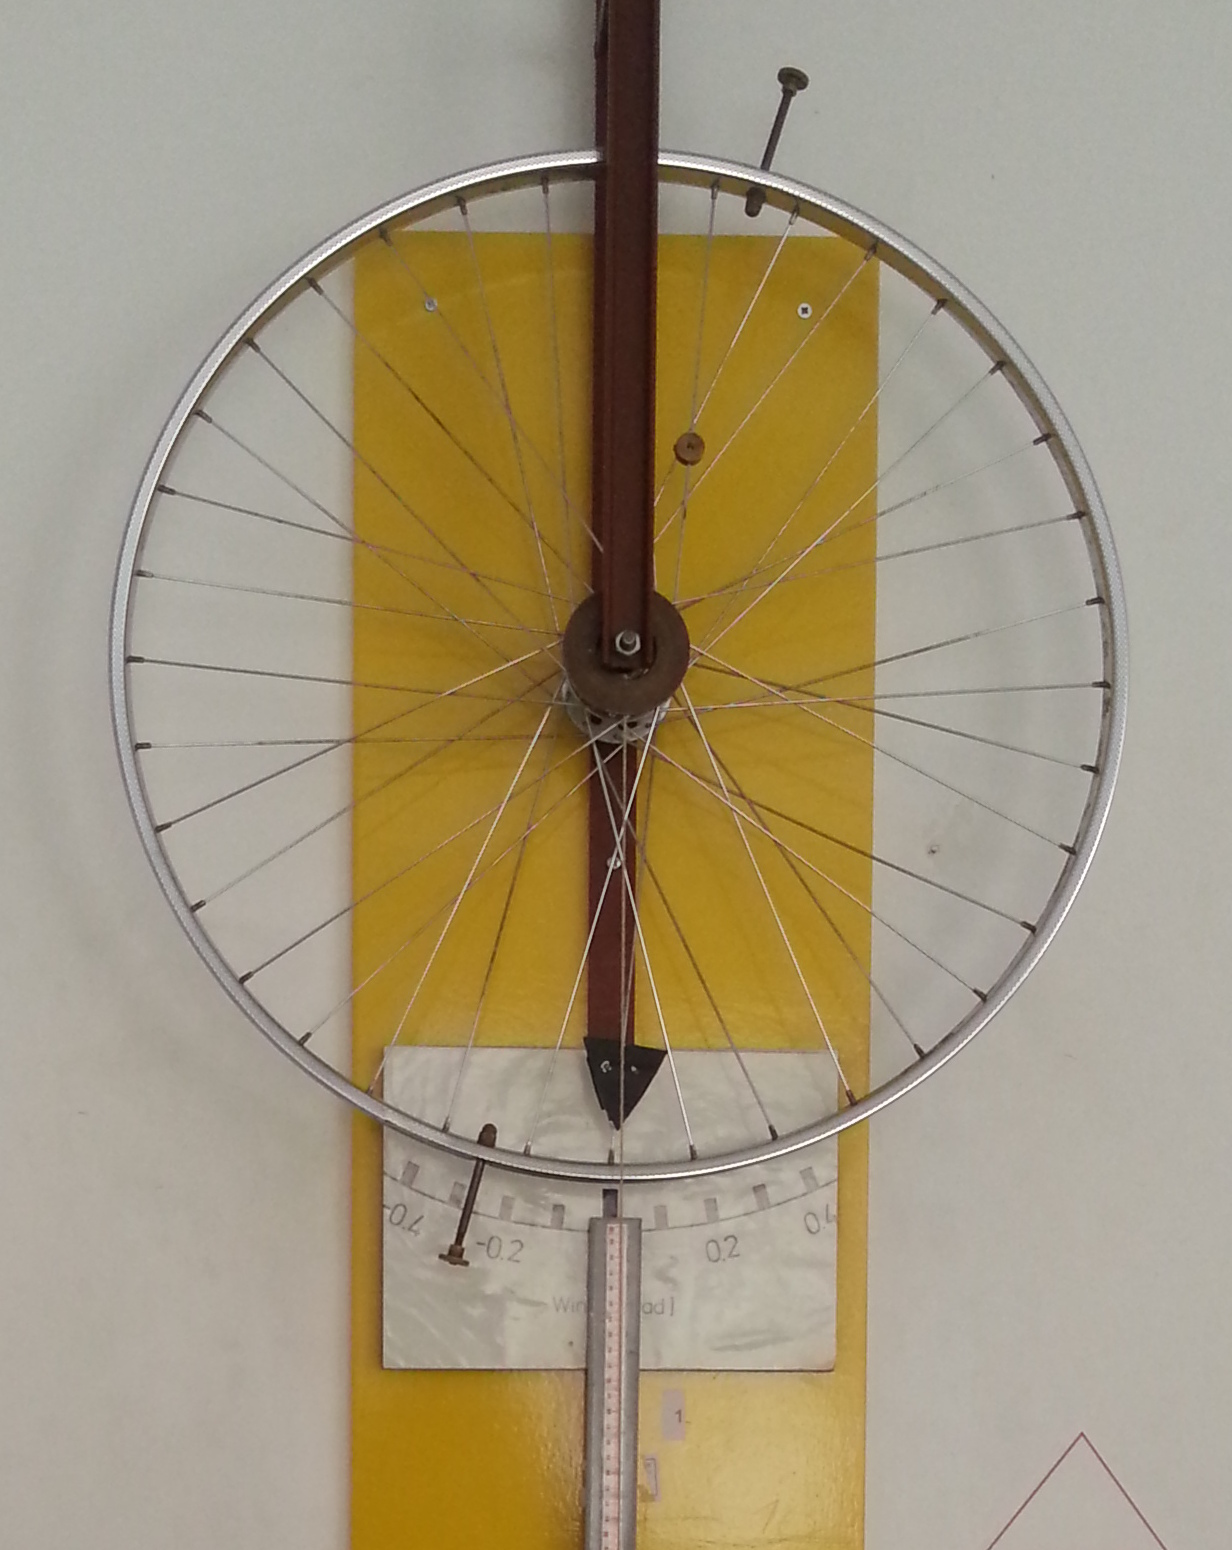
\includegraphics[width=10cm]{fig1.jpg}};
    \draw[red,ultra thick] (5.1,11.2) circle (0.5); % center top
    \draw[red,ultra thick] (2.8,10.7) circle (0.5); % left top
    \draw[red,ultra thick] (7.2,10.7) circle (0.5); % right top
    \draw[red,ultra thick] (5.1,7.4) circle (0.5);  % axis
    \draw[red,ultra thick] (2.8,3.7) circle (0.5);  % left bottom
    \draw[red,ultra thick] (7.2,3.7) circle (0.5);  % right bottom
  \end{tikzpicture}
  \caption{Trackingpunkte für die Ausrichtung}
\end{wrapfigure}
Um stets eine konstante Ausrichtung zu erhalten und zu wissen, wie des Video
gegenüber dem Aufbau rotiert und translatiert ist, muss die Orientierung
konstant gehalten werden.  Dazu werden zuerst im Video über ein statisches
Matching sechs feste Punkte erkannt, um die Orientierung des Experiments
gegenüber der Kamera zu berechnen. Folgende Punkte (siehe Abbildung 1) haben
sich dabei als gut erkennbar herausgestellt:
\begin{enumerate}
  \item Die linke obere Ecke des gelben Hintergrunds
  \item Die rechte obere Ecke des gelben Hintergrunds
  \item Der obere Punkt, bei dem das Rad hinter dem Träger verschwindet
  \item Die Drehachse des Rades
  \item Der linke untere Punkt an dem das Rad den gelben Hintergrund verlässt
  \item Der rechte untere Punkt an dem das Rad den gelben Hintergrund verlässt
\end{enumerate}

Konkret werden dabei Bilder der einzelnen Punkte über das Video bewegt und die
jeweilige Korrelation mit dem Hintergrund berechnet. Dort wo sich das Maximum
der Korrelation befindet, befindet sich der Punkt. Das Verfahren ist dabei aber
anfällig für zweierlei Störungen. Wenn der Punkt überdeckt wird, wird er
irgendwo anders gefunden, dies muss erkannt und herausgefiltert werden. Auch
mit sich ändernden Lichtverhältnissen gibt es Probleme, z.B. wenn die Sonne auf
das Rad scheint und es reflektiert. Dafür ist der Algorithmus erstaunlich
unempfindlich gegen Bewegungsunschärfe.

\subsection{Positionsbestimmung des Zeigers durch direkte Erkennung}
\begin{wrapfigure}{L}{10.1 cm}
  \begin{tikzpicture}
    \node[anchor=south west,inner sep=0] at (0,0) {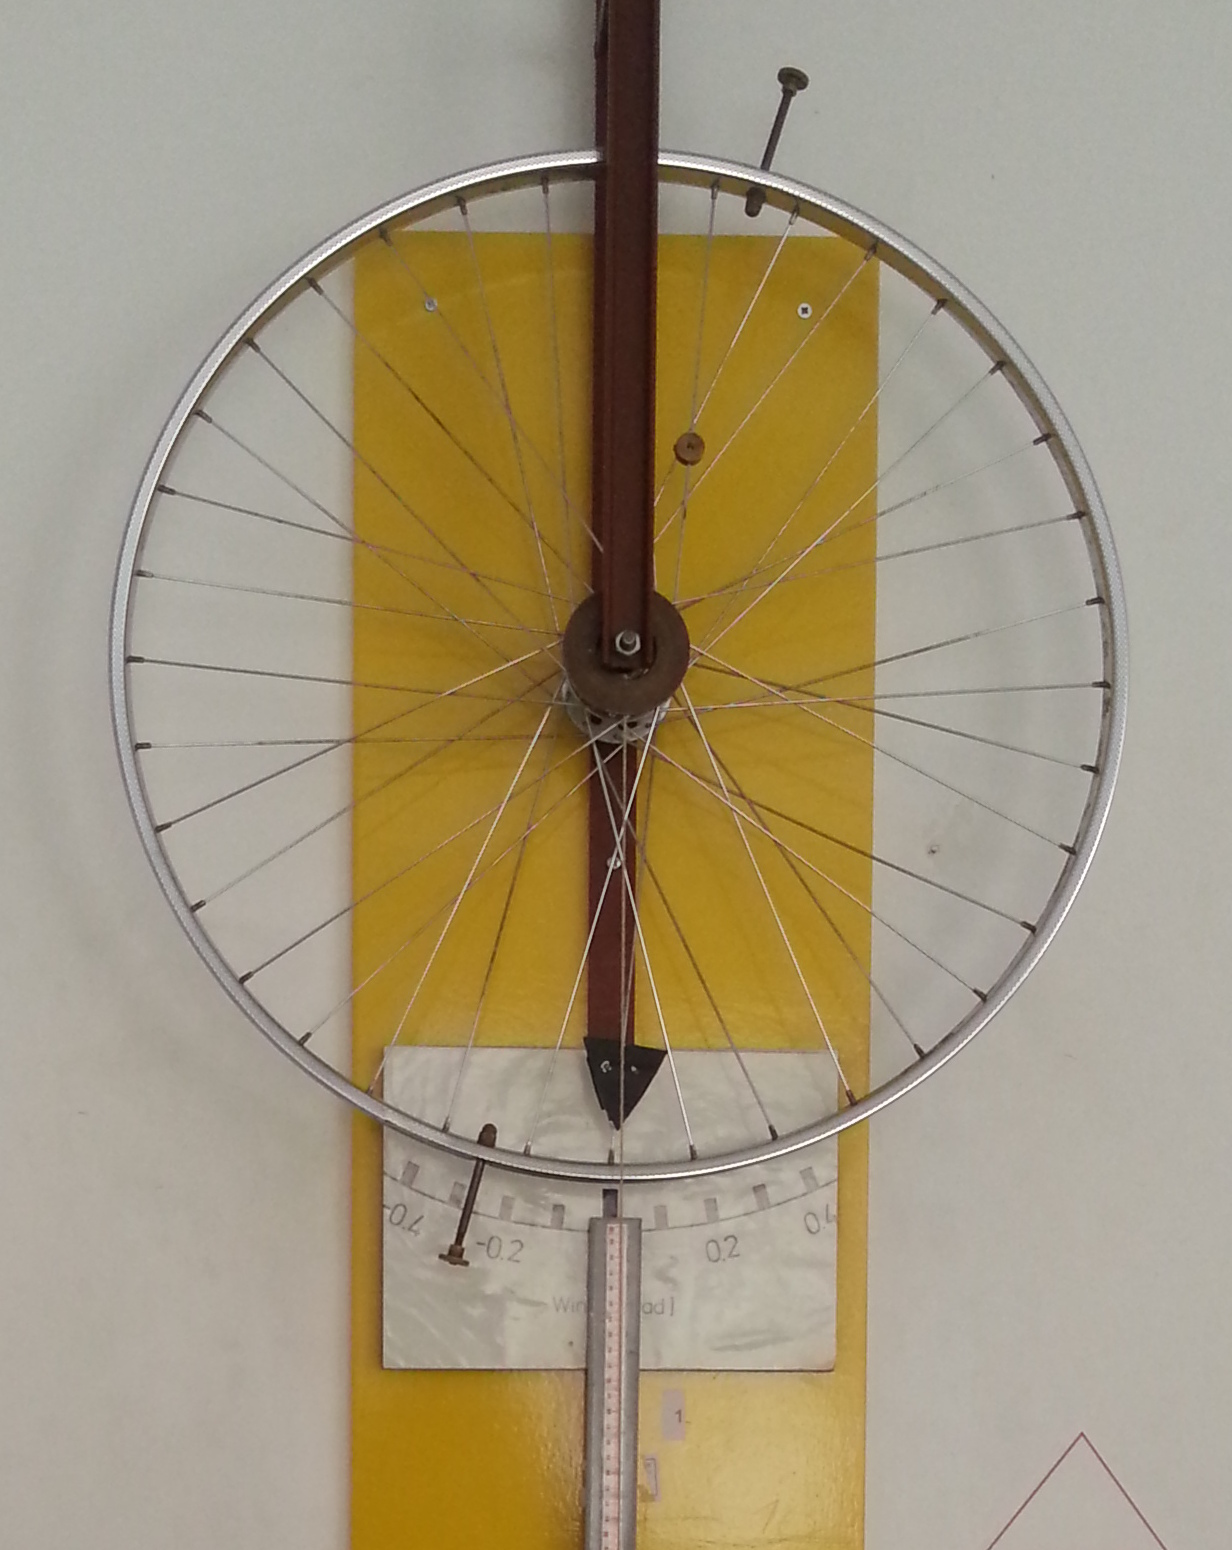
\includegraphics[width=10cm]{fig1.jpg}};
    \draw[red,ultra thick] (1.1,9.4) rectangle (2.1,4.7);  % left
    \draw[red,ultra thick] (7.9,9.4) rectangle (8.9,4.7);  % right
    \draw[red,ultra thick] (3.4,4.3) rectangle (6.6,3.1);  % center
  \end{tikzpicture}
  \label{zones}
  \caption{Zonen für die Erkennung}
\end{wrapfigure}
Sofern der Zeiger in einer von drei verschiedenen Zonen (siehe Abbildung 3) ist,
wird die Position direkt mithilfe der Methode von oben erkannt. Problematisch
sind dabei Rotationen, so dass für jede Zone ein jeweils anderes Bild des
Zeigers verwendet werden muss. Die Methode funktioniert nicht mehr, sobald der
Zeiger einen anderen Hintergrund überstreicht oder seine Orientierung stark
ändert, so dass in diesen Positionen auf andere Methoden zurückgegriffen werden
muss.

\subsection{Indirekte Erkennung der Rotation des Rades}
Sofern der Zeiger nicht innerhalb einer der Zonen ist wird stattdessen direkt
die Rotation des Rades bestimmt. Dazu läuft in gewissen Abständen eine
Erkennung starker Pixelgradienten über definierte Zonen vor ruhigem Hintergrund
(sog. Edge Detection). So werden bis zu 20 Punkte gefunden, die zum Rad
gehören. Dann wird mit dem nächsten Frame verglichen und versucht, die Punkte
dort wiederzufinden. Somit ist bekannt, welcher Punkt sich im Vergleich zum
nächsten Frame wohin bewegt hat. Über die Abschätzung einer
Transformationsmatrix zwischen den Punkten kann dann der Winkel bestimmt werden
um den sich das Rad gedreht hat.

Problematisch an dieser Methode ist, dass sie starke Gradienten, also klare
Ecken vorraussetzt. Bei schnellen Bewegungen wird der Fehler schnell sehr groß
bzw. es werden überhaupt keine Ecken mehr gefunden, die getrackt werden können.
Dann muss gewartet werden, bis der Zeiger wieder in einer der Zonen ist, um die
Position wiederzufinden.

\subsection{Ausgabe}
Einerseits schreibt das Programm die berechneten Werte direkt in eine CSV-Datei, andererseits wird auch ein Video generiert, dass die Position des Zeigers direkt mit Fehlerbalken, Werten und Zeitindex anzeigt um die Funktionsweise zu prüfen.

\subsection{Implementierung und Performance}
Die Software wurde in C geschrieben und benutzt die OpenCV-Bibliothek, die die
Grafikfunktionalitäten zur Verfügung stellt. Es hat einen Umfang von knapp 800
Zeilen und benötigt auf meinem Laptop etwa 16 Stunden um alle 60 Videos zu
bearbeiten.

\subsection{Weitere Auswertung}
Die CSV-Daten werden anschließend mit einem weiteren Programm bearbeitet,
welches die Werte zwischen Start- und Umkehrpunkt herausschneidet und dabei den
Nullpunkt festsetzt. Außerdem gibt es noch diverse Hilfsprogramme in Ruby. Hier
wurden insgesamt 200 Zeilen Code geschrieben. Außerdem über 1000 Zeilen
GNUplot-Code, der aber größtenteils von den Hilfsprogrammen generiert wird.

\section{Zusammenfassung und Diskussion}
Insgesamt konnten wir dank rechnergestützter Auswertung das hergeleitete
Bewegungsgesetz wiederlegen. Erst ein Ansatz mit einer
geschwindigkeitsabhängigen Reibung kann die Bewegung des Rades näherungsweise
erklären, auch wenn an einigen Stellen (z.B. Messung 60) der Einfluss einer
nichtlinearen Reibung klar erkannbar sind. Gerade für die letzten Messungen
konnten wir keine Werte aufnehmen, da das Rad sich nicht bewegt hat. Hierbei
handelt es sich um eine Haftreibung.

Aus den Differenzen der Laufzeiten für Links- und Rechtsdrehung ist außerdem
ersichtlich, dass das Rad Unwuchten hat, die das Ergebnis weiter verfälschen.

Aufgrund dieser konstruktionsbedingten Ungenauigkeiten im Aufbau konnten wir
die Trägheitsmomente leider nicht in der gewünschten Genauigkeit berechnen,
dennoch konnten wir die Gültigkeit des Steinerschen Satzes zeigen.


Da für die Messungen die nicht mit der Software auswertbar waren, jeweils nur
zwei Messpunkte verfügbar sind, können nicht alle Parameter der
Bewegungsgleichung ermittelt werden. Deswegen mussten wir diese Messungen
vernachlässigen.

Mit einer verbesserten Software wäre dies sicherlich möglich, aber da wir ein
breites Spektrum an Messungen über alle Parameter auswerten konnten, bringt
dies wahrscheinlich keine neuen Erkenntnisse. Deswegen lassen wir das.


\invisiblesection{Grafische Auswertungen und Wertetabellen}

\newpage
\begin{landscape}
  % gnuplot ./plot/plot-57-quad.gnuplot
  \input{plot-57-quad.tex}
\end{landscape}

\newpage
\begin{landscape}
  % gnuplot ./plot/plot-41-exp.gnuplot
  \input{plot-41-exp.tex}
\end{landscape}

\newpage
\begin{landscape}
  % gnuplot ./plot/plot-34-exp.gnuplot
  \input{plot-34-exp.tex}
\end{landscape}

\newpage
\begin{landscape}
  % gnuplot ./plot/plot-24-exp.gnuplot
  \input{plot-24-exp.tex}
\end{landscape}

\newpage
\begin{landscape}
  % gnuplot ./plot/plot-20-exp.gnuplot
  \input{plot-20-exp.tex}
\end{landscape}

\newpage
\begin{landscape}
  % gnuplot ./plot/plot-8-exp.gnuplot
  \input{plot-8-exp.tex}
\end{landscape}

\newpage
\begin{landscape}
  % gnuplot ./plot/plot-1-exp.gnuplot
  \input{plot-1-exp.tex}
\end{landscape}

\newpage
\begin{landscape}
  % gnuplot ./plot/plot-13-exp.gnuplot
  \input{plot-13-exp.tex}
\end{landscape}

\newpage
\begin{landscape}
  % gnuplot ./plot/plot-16-exp.gnuplot
  \input{plot-16-exp.tex}
\end{landscape}

\newpage
\begin{landscape}
  % gnuplot ./plot/plot-14-exp.gnuplot
  \input{plot-14-exp.tex}
\end{landscape}

\newpage
\begin{landscape}
  % gnuplot ./plot/plot-57-exp.gnuplot
  \input{plot-57-exp.tex}
\end{landscape}

\newpage
\begin{landscape}
  % gnuplot ./plot/plot-12-exp.gnuplot
  \input{plot-12-exp.tex}
\end{landscape}

\newpage
\begin{landscape}
  % gnuplot ./plot/plot-19-exp.gnuplot
  \input{plot-19-exp.tex}
\end{landscape}

\newpage
\begin{landscape}
  % gnuplot ./plot/plot-10-exp.gnuplot
  \input{plot-10-exp.tex}
\end{landscape}

\newpage
\begin{landscape}
  % gnuplot ./plot/plot-47-exp.gnuplot
  \input{plot-47-exp.tex}
\end{landscape}

\newpage
\begin{landscape}
  % gnuplot ./plot/plot-22-exp.gnuplot
  \input{plot-22-exp.tex}
\end{landscape}

\newpage
\begin{landscape}
  % gnuplot ./plot/plot-55-exp.gnuplot
  \input{plot-55-exp.tex}
\end{landscape}

\newpage
\begin{landscape}
  % gnuplot ./plot/plot-4-exp.gnuplot
  \input{plot-4-exp.tex}
\end{landscape}

\newpage
\begin{landscape}
  % gnuplot ./plot/plot-46-exp.gnuplot
  \input{plot-46-exp.tex}
\end{landscape}

\newpage
\begin{landscape}
  % gnuplot ./plot/plot-5-exp.gnuplot
  \input{plot-5-exp.tex}
\end{landscape}

\newpage
\begin{landscape}
  % gnuplot ./plot/plot-21-exp.gnuplot
  \input{plot-21-exp.tex}
\end{landscape}

\newpage
\begin{landscape}
  % gnuplot ./plot/plot-31-exp.gnuplot
  \input{plot-31-exp.tex}
\end{landscape}

\newpage
\begin{landscape}
  % gnuplot ./plot/plot-60-exp.gnuplot
  \input{plot-60-exp.tex}
\end{landscape}

\newpage
\begin{landscape}
  % gnuplot ./plot/plot-40-exp.gnuplot
  \input{plot-40-exp.tex}
\end{landscape}

\newpage
\begin{landscape}
  % gnuplot ./plot/plot-6-exp.gnuplot
  \input{plot-6-exp.tex}
\end{landscape}

\newpage
\begin{landscape}
  % gnuplot ./plot/plot-49-exp.gnuplot
  \input{plot-49-exp.tex}
\end{landscape}

\newpage
\begin{landscape}
  % gnuplot ./plot/plot-52-exp.gnuplot
  \input{plot-52-exp.tex}
\end{landscape}

\newpage
\begin{landscape}
  % gnuplot ./plot/plot-17-exp.gnuplot
  \input{plot-17-exp.tex}
\end{landscape}

\newpage
\begin{landscape}
  % gnuplot ./plot/plot-9-exp.gnuplot
  \input{plot-9-exp.tex}
\end{landscape}

\newpage
\begin{landscape}
  % gnuplot ./plot/plot-3-exp.gnuplot
  \input{plot-3-exp.tex}
\end{landscape}

\newpage
\begin{landscape}
  % gnuplot ./plot/plot-54-exp.gnuplot
  \input{plot-54-exp.tex}
\end{landscape}

\newpage
\begin{landscape}
  % gnuplot ./plot/plot-53-exp.gnuplot
  \input{plot-53-exp.tex}
\end{landscape}

\newpage
\begin{landscape}
  % gnuplot ./plot/plot-15-exp.gnuplot
  \input{plot-15-exp.tex}
\end{landscape}



\begin{tabular}{l|r|r|r|r|r}
Messung & $A$ & $B$ & $C$ & $I$ & $\mu$ \\
1 & $\num{9.3+-0.31}$ & $\num{0.198+-0.0044}$ & $\num{1.86+-0.023}$, & $\num{0.83+-0.018}$ & $\num{0.165+-0.0021}$ \\
3 & $\num{14.2+-0.98}$ & $\num{0.162+-0.008}$ & $\num{2.31+-0.058}$, & $\num{0.82+-0.039}$ & $\num{0.133+-0.0033}$ \\
4 & $\num{200+-19.0}$ & $\num{0.039+-0.0027}$ & $\num{6.0+-0.34}$, & $\num{1.3+-0.16}$ & $\num{0.051+-0.003}$ \\
5 & $\num{120+-4.6}$ & $\num{0.045+-0.001}$ & $\num{5.43+-0.088}$, & $\num{1.25+-0.043}$ & $\num{0.0567+-0.00094}$ \\
6 & $\num{300+-11.0}$ & $\num{0.0283+-0.00062}$ & $\num{7.6+-0.13}$, & $\num{1.42+-0.059}$ & $\num{0.0406+-0.00075}$ \\
8 & $\num{1000+-280.0}$ & $\num{0.033+-0.0087}$ & $\num{20+-4.4}$, & $\num{0+-1.2}$ & $\num{0.04+-0.01}$ \\
9 & $\num{60+-3.7}$ & $\num{0.115+-0.0042}$ & $\num{6.8+-0.18}$, & $\num{0.94+-0.07}$ & $\num{0.11+-0.003}$ \\
10 & $\num{400+-54.0}$ & $\num{0.041+-0.0034}$ & $\num{10+-1.1}$, & $\num{1.2+-0.31}$ & $\num{0.051+-0.0037}$ \\
12 & $\num{600+-38.0}$ & $\num{0.0301+-0.00095}$ & $\num{19.4+-0.53}$, & $\num{1.3+-0.14}$ & $\num{0.038+-0.0012}$ \\
13 & $\num{50+-4.9}$ & $\num{0.169+-0.0093}$ & $\num{8.4+-0.37}$, & $\num{1.0+-0.13}$ & $\num{0.175+-0.0077}$ \\
14 & $\num{20+-3.5}$ & $\num{0.34+-0.048}$ & $\num{4.9+-0.46}$, & $\num{0.8+-0.21}$ & $\num{0.3+-0.028}$ \\
15 & $\num{500+-43.0}$ & $\num{0.051+-0.0024}$ & $\num{24+-1.0}$, & $\num{1.2+-0.23}$ & $\num{0.062+-0.0028}$ \\
16 & $\num{100+-19.0}$ & $\num{0.104+-0.0083}$ & $\num{13.5+-0.88}$, & $\num{1.0+-0.25}$ & $\num{0.109+-0.0072}$ \\
17 & $\num{600+-55.0}$ & $\num{0.044+-0.002}$ & $\num{30+-1.1}$, & $\num{1.2+-0.23}$ & $\num{0.052+-0.0023}$ \\
19 & $\num{100+-25.0}$ & $\num{0.12+-0.013}$ & $\num{10+-1.4}$, & $\num{1.1+-0.39}$ & $\num{0.14+-0.013}$ \\
20 & $\num{100+-27.0}$ & $\num{0.14+-0.022}$ & $\num{10+-1.7}$, & $\num{1.1+-0.51}$ & $\num{0.16+-0.021}$ \\
21 & $\num{100+-21.0}$ & $\num{0.113+-0.009}$ & $\num{20+-1.1}$, & $\num{1.0+-0.28}$ & $\num{0.124+-0.0083}$ \\
22 & $\num{1000+-200.0}$ & $\num{0.043+-0.0049}$ & $\num{40+-4.1}$, & $\num{1.2+-0.74}$ & $\num{0.053+-0.0059}$ \\
24 & $\num{1000+-190.0}$ & $\num{0.033+-0.0023}$ & $\num{50+-3.0}$, & $\num{1.2+-0.48}$ & $\num{0.042+-0.0029}$ \\
31 & $\num{80+-7.8}$ & $\num{0.095+-0.005}$ & $\num{7.7+-0.34}$, & $\num{3.6+-0.24}$ & $\num{0.35+-0.015}$ \\
34 & $\num{1000+-170.0}$ & $\num{0.031+-0.004}$ & $\num{20+-2.5}$, & $\num{0+-1.1}$ & $\num{0.13+-0.015}$ \\
40 & $\num{100+-20.0}$ & $\num{0.062+-0.0046}$ & $\num{9.0+-0.56}$, & $\num{3.6+-0.36}$ & $\num{0.23+-0.014}$ \\
41 & $\num{1000+-130.0}$ & $\num{0.019+-0.001}$ & $\num{30+-1.2}$, & $\num{4.1+-0.48}$ & $\num{0.081+-0.004}$ \\
46 & $\num{1000+-190.0}$ & $\num{0.019+-0.002}$ & $\num{20+-1.7}$, & $\num{4.3+-0.86}$ & $\num{0.082+-0.008}$ \\
47 & $\num{1100+-91.0}$ & $\num{0.0181+-0.00082}$ & $\num{19.4+-0.78}$, & $\num{4.2+-0.36}$ & $\num{0.076+-0.0032}$ \\
49 & $\num{20+-1.7}$ & $\num{0.102+-0.0043}$ & $\num{2.44+-0.074}$, & $\num{2.97+-0.085}$ & $\num{0.306+-0.0093}$ \\
52 & $\num{1000+-250.0}$ & $\num{0.013+-0.0016}$ & $\num{10+-1.5}$, & $\num{4.6+-0.93}$ & $\num{0.058+-0.007}$ \\
53 & $\num{500+-25.0}$ & $\num{0.0182+-0.00047}$ & $\num{9.7+-0.21}$, & $\num{4.2+-0.14}$ & $\num{0.077+-0.0018}$ \\
54 & $\num{1100+-59.0}$ & $\num{0.0122+-0.00034}$ & $\num{13.6+-0.34}$, & $\num{4.5+-0.2}$ & $\num{0.055+-0.0015}$ \\
55 & $\num{30+-2.2}$ & $\num{0.051+-0.0021}$ & $\num{1.78+-0.045}$, & $\num{3.39+-0.065}$ & $\num{0.173+-0.0044}$ \\
57 & $\num{21.5+-0.69}$ & $\num{0.069+-0.0015}$ & $\num{1.48+-0.019}$, & $\num{2.98+-0.028}$ & $\num{0.208+-0.0026}$ \\
60 & $\num{2000+-530.0}$ & $\num{0.0052+-0.00072}$ & $\num{10+-1.3}$, & $\num{6+-1.0}$ & $\num{0.031+-0.004}$ \\
\end{tabular}

\end{document}
